%!TEX root = ../thesis.tex
%******************************************************************************
\chapter{Performance Evaluation of Batch and Message-based Systems}\label{ch:performance_evaluation}
%******************************************************************************

\section{Introduction}\label{sec:ch4_introduction}

Traditionally, business information systems for bulk data processing are implemented as batch processing systems. Batch processing delivers high throughput but cannot provide near-time processing of data, that is the end-to-end latency of such a system is high. 

A lower end-to-end latency can be achieved by using message-based processing, for example by utilising a message-oriented middleware for the integration of the services that form the business information system. While this approach is able to deliver near-time processing, it is hardly capable for bulk data processing due to the additional communication over- head for each processed message. Therefore, message-based processing is ususally not considered for building a system for bulk data processing requiring high throughput.

This chapter compares the performance of a batch and message-based system. The main objectives of this comparison are:

\begin{itemize}
  \item What is the impact of different processing styles, that is batch and message-based processing, on throughput and latency?
  \item What is the impact of data granularity on latency and throughput when using a message-based processing style?  
\end{itemize}

To find solutions for these questions, the following approach has been taken:

\begin{itemize}
	\item Two prototypes of a billing system for each processing type (see Section \ref{sec:ch4_prototype}) have been built. 
	\item A performance evaluation has been conducted to compare the prototypes with each other with the focus on throughput and latency (see Section \ref{sec:ch4_evaluation}).
	\item To evaluate the impact of different aggregatation sizes on throughput and latency, the messaging prototype has been extended with an aggregator. A performance test has been conducted with different static aggregation sizes (see Section \ref{sec:ch4_impact_granularity}).
\end{itemize}

This chapter is organised as follows. Section \ref{sec:ch4_prototype} introduces the batch and message-based prototype systems that have been implemented. To compare the performance characterics of the two processing types, batch processing and message-based processing, a performance evaluation has been conducted, which is presented in Section \ref{sec:ch4_evaluation}. Section \ref{sec:ch4_impact_granularity} shows the impact of data granularity on throughput and latency of the messaging prototype. Section \ref{sec:ch4_related_work} gives an overview of other work related to the contents of this chapter. Finally, this chapter concludes with a summary in Section \ref{sec:ch4_summary} 

\section{A real world example  application}\label{sec:ch4_prototype}
This section introduces the two prototypes of a billing system that have been built to evaluate the performance of batch and message-based processing.

A billing system is a distributed system consisting of several sub components that process the different billing sub processes like mediation, rating, billing and presentment (see Figure \ref{fig:ch4_billing_process}).

\begin{figure}[h!]
	\centering
	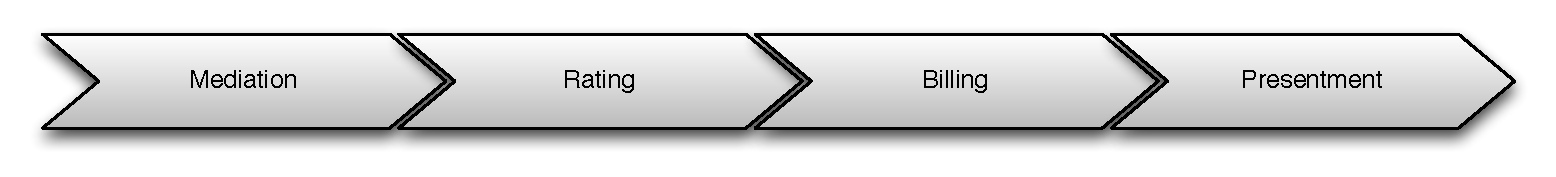
\includegraphics[width=\columnwidth]{billing_process}
	\caption{Billing process}
	\label{fig:ch4_billing_process}
\end{figure}

The mediation components receive usage events from delivery systems, like switches and transform them into a format the billing system is able to process. For example, transforming the event records to the internal record format of the rating and billing engine or adding internal keys that are later needed in the process. The rating engine assigns the events to the specific customer account, called guiding, and determines the price of the event, depending on the applicable tariff. It also splits events if more than one tariff is applicable or the customer qualifies for a discount. The billing engine calculates the total amount of the bill by adding the rated events, recurring and one-time charges and discounts. The output is processed by the presentment components, which format the bill, print it, or present it to the customer in self-service systems, for example on a website.

In order to compare batch and message-based types of processing, two different prototypes of a billing application have been developed. Each prototype implements the mediation and rating steps of the billing process. Figure \ref{fig:ch4_prototype_components} shows the components of the billing prototype: 
\begin{itemize}
	\item \textbf{Event Generator}\\
	The \emph{Event Generator} generates the calling events, i.e. the \ac{CDR} that are processed by the billing application.
	\item \textbf{Mediation}\\
	The \emph{Mediation} component checks wether the calltime of the calldetail record exceeds the minimal billable length or if it belongs to a flatrate account and sets the corresponding flags of the record. The output of the \emph{Mediation} component are \ac{NCDR} that are further processed by the \emph{Rating} component.
	\item \textbf{Rating}\\
	The \emph{Rating} component processes the output from the \emph{Mediation} component. It assigns the calldetail record to a customer account and determines the price of the call event by looking up the correspondant product and tariff in the \emph{Master Data DB}. The output of the \emph{Rating} component (costed events) is afterwards written to the \emph{Costed Events DB}.
	\item \textbf{Master Data DB}\\
	The \emph{Master Data DB} contains products, tariffs and accounts used by the \emph{Event Generator} and the \emph{Rating} component.
	\item \textbf{Costed Events DB}\\
	The \emph{Costed Events DB} contains the result of the \emph{Rating} component, i.e. the costed events.
\end{itemize}

\begin{figure}[h!]
	\centering
	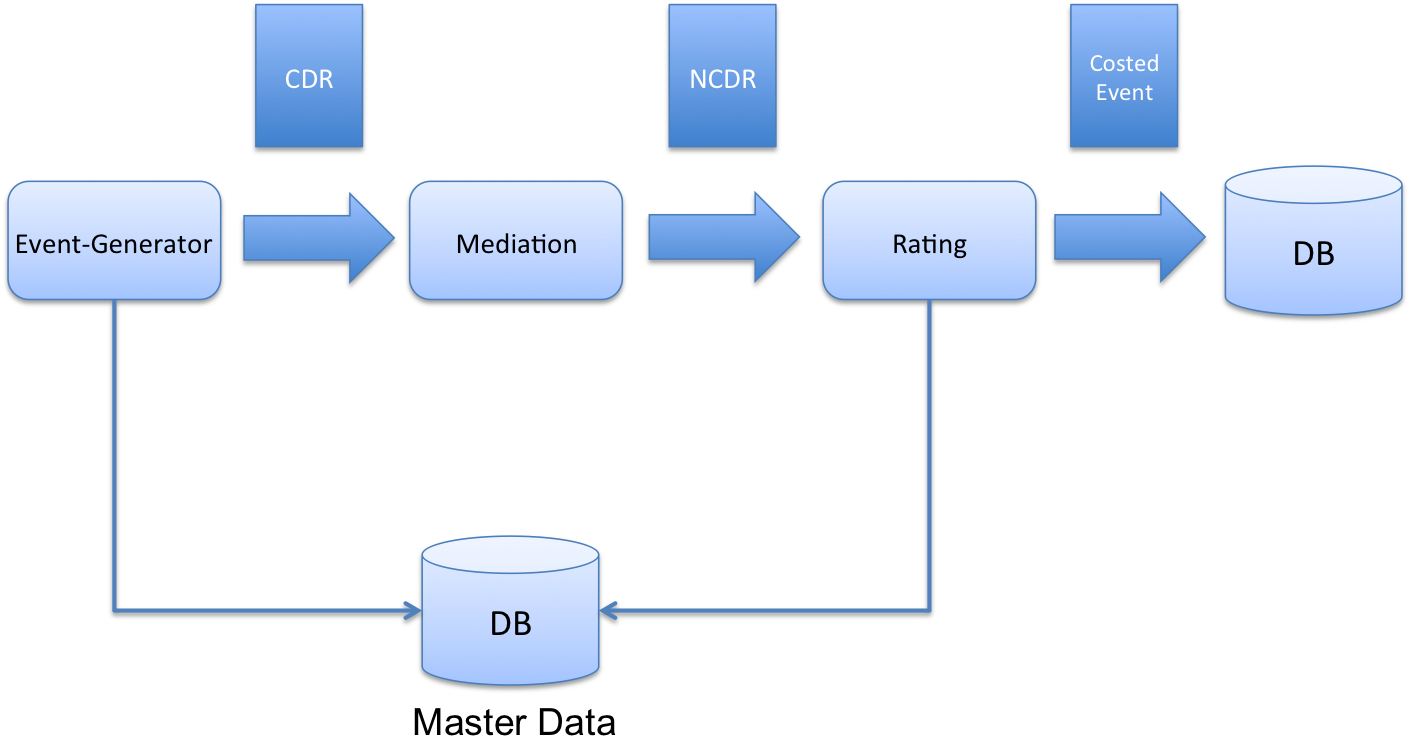
\includegraphics[width=\columnwidth]{prototype_components}
	\caption{Components of the billing application prototype}
	\label{fig:ch4_prototype_components}
\end{figure}

The prototypes are implemented with Java 1.6 using \ac{JPA} for the data-access layer and a MySQL database. To ensure comparability, the prototypes share the same business components, database and data-access layer, varying only in different integration layers (see Figure \ref{fig:ch4_technical_integration}). 

\begin{figure}[h!]
	\centering
	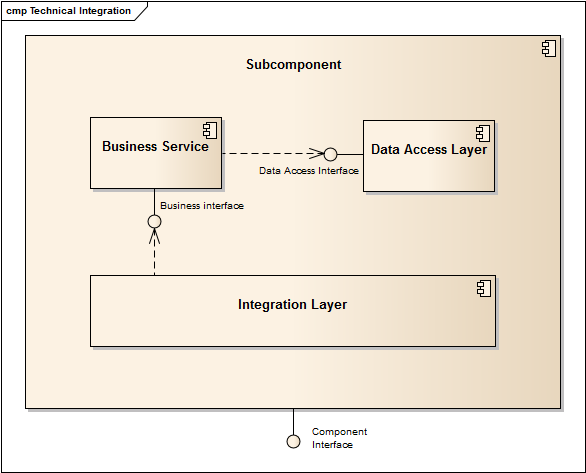
\includegraphics[width=\columnwidth]{technical_integration}
	\caption{The prototypes share the same business components, database and data-access layer.}
	\label{fig:ch4_technical_integration}
\end{figure}

\subsection{Batch prototype}
The batch prototype implements the billing application utilizing the batch processing type. It uses the Spring Batch framework \citep{springbatch}, a Java framework that facilitates the implementation of batch applications by providing basic building blocks for reading, writing and processing data.

Figure \ref{fig:ch4_batch_prototype} shows the architecture of the batch prototype. It consists of two nodes, mediation batch and rating batch, each implemented as a separate spring batch application. The nodes are integrated using Apache Camel \citep{apachecamel}, an Java integration framework based on enterprise integration patterns, as described by \cite{Hohpe:2003fk}. Apache Camel is responsible for listening on the file system, calling the Spring batch application when a file arrives and transferring the output from the mediation batch node to the rating batch node using \ac{FTP}.

\begin{figure}[h!]
	\centering
	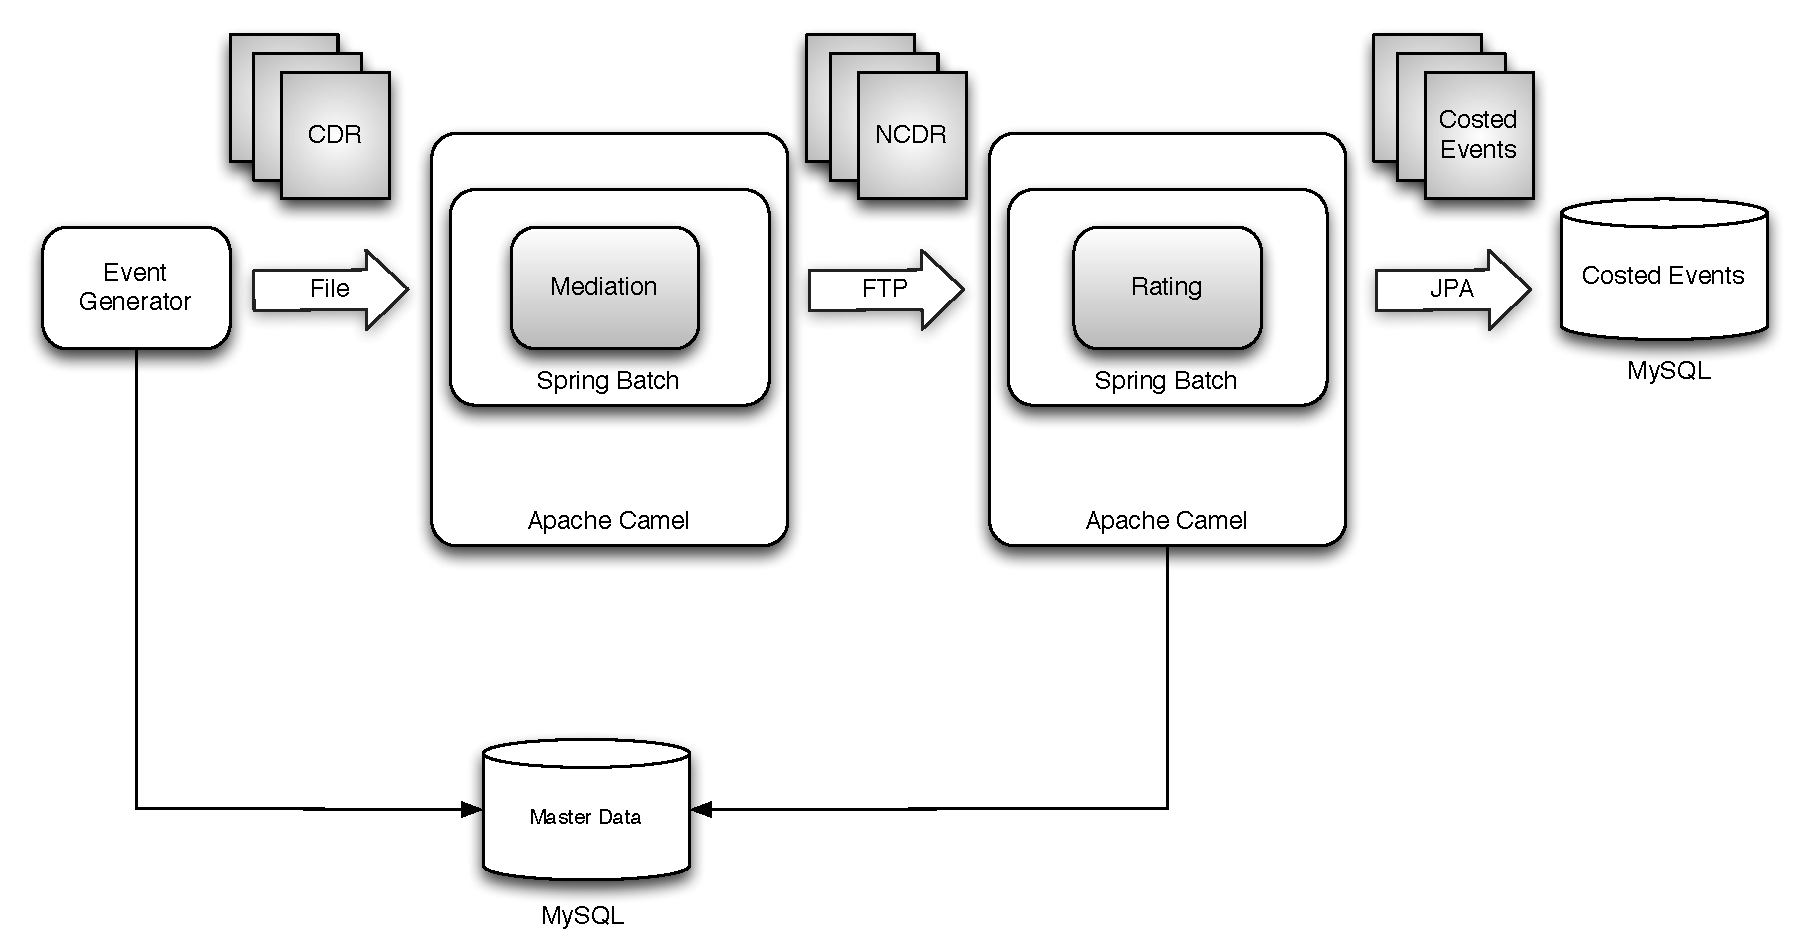
\includegraphics[width=\columnwidth]{batch_prototype}
	\caption{Batch prototype}
	\label{fig:ch4_batch_prototype}
\end{figure}

The batch prototype performs the following steps:
\begin{enumerate}
	\item The \emph{Event generator} generates call detail records and writes them to a single file.
	\item The \emph{Mediation component} opens the file, processes it and writes the output to a single output file. The output file is getting transfered using \ac{FTP} to the \emph{Rating component}.
	\item The \emph{Rating component} opens the file, processes it and writes the costed events to the costed event database.
\end{enumerate}

\subsubsection{Implementation details}
The main entities in Spring Batch are Jobs and Steps. A Job defines the processing flow of the batch application and consists of one or more steps. A basic step is comprised of an item reader, item processor and item writer (see Figure \ref{fig:ch4_spring_batch_step}). 
\begin{figure}[h!]
	\centering
	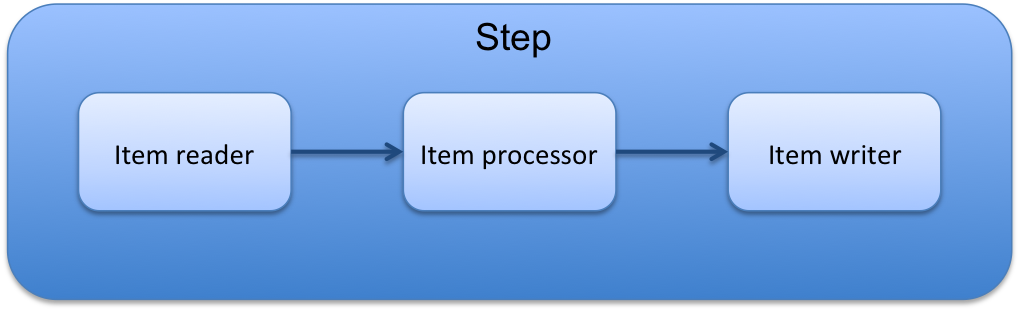
\includegraphics[width=\columnwidth]{spring_batch_step}
	\caption{A Step consists of an item reader, item processor and item writer}
	\label{fig:ch4_spring_batch_step}
\end{figure}

The item reader reads records of data in chunks, for example from a file, and converts them to objects. These objects are then processed by the item processor, which contains the business logic of the batch application. Finally, the processed objects are getting written to the output destination, for example a database, by the item writer.

\lstinputlisting[caption={Mediation batch job definition},label=listing:ch4_mediation_job]{listings/mediation_job.xml}

Listing \ref{listing:ch4_mediation_job} shows the definition of the mediation batch job \emph{mediationMultiThreadedJob}. It consists of two steps, the \emph{mediationMultiThreadedStep} (line 2) and the \emph{renameFileMultiThreadedStep} (line 10). The step \emph{mediationMultiThreadedStep} is multithreaded and uses 10 threads for processing. It consists of a \emph{rawUsageMultiThreadedEventReader} (line 6), a thread safe reader implementation that reads call detail records from the input file and converts them to objects, a \emph{rawUsageEventProcessor}, that processes the call detail objects by calling the mediation business logic and a \emph{loggingSimpleCdrWriter} (line 7), which writes the processed call detail objects to the output file. The step uses an commit interval of 1000, meaning that the input data is processed in chunks of 1000 records. After the input file has been processed by the \emph{mediationMultiThreadedStep} it is getting renamed to its final name by the \emph{renameFileMultiThreadedStep} (line 10).

The mediation batch job is integrated using Apache Camel. Listing \ref{listing:ch4_mediation_route} shows the definition of the mediation batch route.

\begin{lstlisting}[caption={Mediation batch route definition},label=listing:ch4_mediation_route]
public void configure() {
	from("file:data/input")
	.to("spring-batch:mediationMultiThreadedJob?jobLauncherRef=jobLauncher");
        
	from("file:data/output)
	.to("ftp://billing@localhost/src/data?password=billing");
}
\end{lstlisting}

It consists of two routes, the first route listens on the file system for incoming files (line 2) and calls the mediation batch job, when a file arrives (line 3). The second route transfers the output file of the mediation batch job to the rating batch node using \ac{FTP} (line 5-6).

Listing \ref{listing:ch4_rating_job} shows the definition of the rating batch job \emph{ratingMultiThreadedJob}. It consists of a single step \emph{ratingMultiThreadedStep} (line 2), which is comprised of a \emph{simpleCdrMultiThreadedItemReader}, which reads the normalized call detail records written by the mediation batch node, a \emph{simpleCdrProcessor}, that processes the normalized call detail records by calling the rating business logic and a \emph{costedEventWriter}, which writes the processed costed events to the Costed Events database (line 4).

\lstinputlisting[caption={Rating batch job definition},label=listing:ch4_rating_job]{listings/rating_job.xml}

\subsection{Messaging prototype}

The messaging prototype implements the billing prototype utilizing the message-oriented processing type. It uses Apache Camel \citep{apachecamel} as the messaging middleware.

Figure \ref{fig:ch4_messaging_prototype} shows the architecture of the messaging prototype. It consists of three nodes, the billing route, mediation service and rating service. The billing route implements the main flow of the application. It is responsible for reading messages from the billing queue, extracting the payload, calling the mediation and rating service and writing the processed messages to the database. The mediation service is a webservice representing the mediation component. It is a SOAP service implemented using Apache CXF and runs inside an Apache Tomcat container. The same applies to the rating service, representing the rating component.

\begin{figure}[h!]
	\centering
	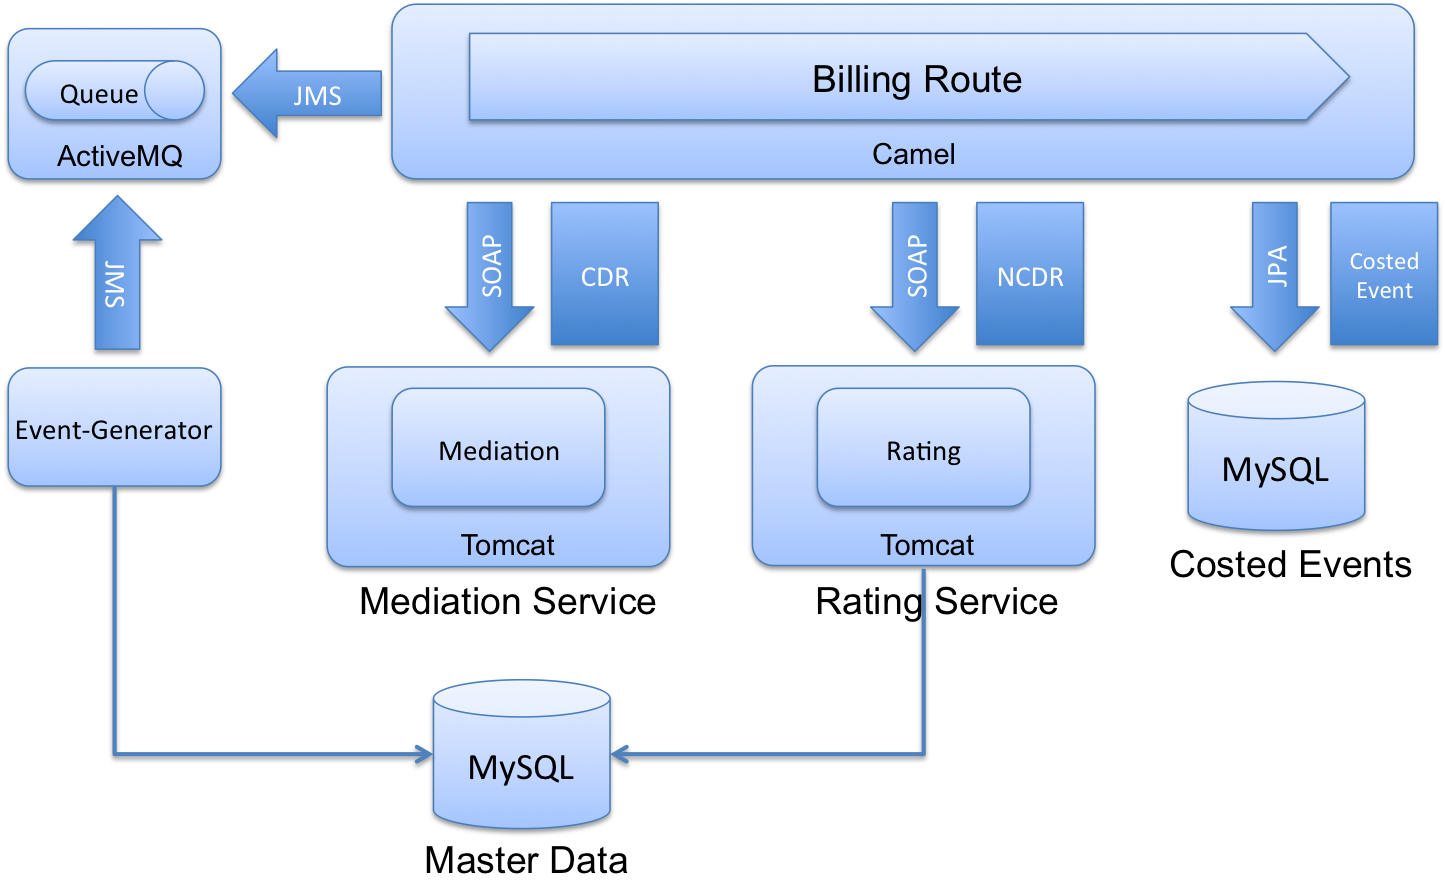
\includegraphics[width=\columnwidth]{messaging_prototype}
	\caption{Message-based prototype}
	\label{fig:ch4_messaging_prototype}
\end{figure}

Listing \ref{listing:ch4_billing_route} shows the definition of the billing route using the Apache Camel fluent \ac{API}.
The billing route performs the following steps:

\begin{enumerate}
	\item The message is read from the billing queue using \ac{JMS} (line 5). The queue ist hosted by an Apache ActiveMQ instance.
	\item The message is unmarshalled using \ac{JAXB} (line 6).
	\item The \emph{Mediation service} is called by the CXF Endpoint of the billing route (line 7)
	\item The response of the \emph{Mediation webservice}, the normalized call detail record, is unmarshalled (line 8). 
	\item The \emph{Rating service} is called by the CXF Endpoint of the billing route (line 9).
	\item The response of the \emph{Rating webservice}, that is the costed event, is unmarshalled (line 10).
	\item The costed event is written to the \emph{Costed Events} DB (line 11).
\end{enumerate}

If an error occurs during the processsing of an event, it is written to an error \ac{JMS} queue (line 3).

\begin{lstlisting}[caption={Billing route definition},label=listing:ch4_billing_route]
public void configure() {
		
	errorHandler(deadLetterChannel("activemq:queue:BILLING.ERRORS"));
	
	from("activemq:queue:BILLING.USAGE_EVENTS")
		.unmarshal("jaxbContext")
		.to("cxf:bean:mediationEndpoint?dataFormat=POJO&defaultOperationName=processEvent")
		.process(new ProcessEventPostProcessor())
		.to("cxf:bean:ratingEndpoint?dataFormat=POJO&defaultOperationName=processCallDetail")
		.process(new ProcessCallDetailPostProcessor())
		.process(costedEventProcessor);
}
\end{lstlisting}

\section{Performance evaluation}\label{sec:ch4_evaluation}
To compare the performance characterics of the two processing types, batch processing and message-based processing, a performance evaluation has been conducted with the main focus on latency and throughput.

This section describes the approach and the results of the performance evaluation.

\subsection{Measuring points}
A number of measuring points have been defined for each prototype by breaking down the processing in single steps and assigning a measuring point to each step. Figure \ref{fig:ch4_measuring_points_batch} and \ref{fig:ch4_measuring_points_messaging} show the measuring points of the batch prototype and the messaging prototype. 

\begin{figure}[htpb]
	\centering
	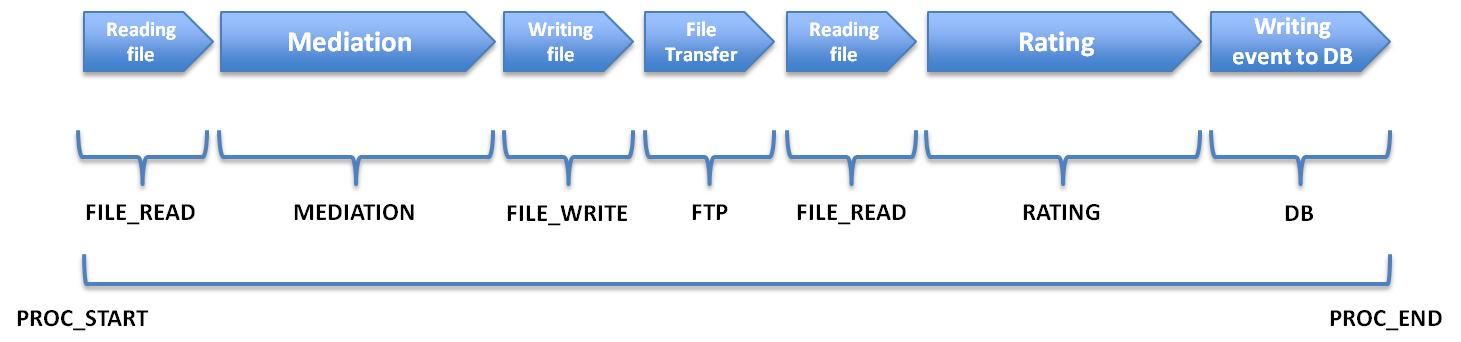
\includegraphics[width=\columnwidth]{measuring_points_batch}
	\caption{Measuring points of the batch prototye}
	\label{fig:ch4_measuring_points_batch}
\end{figure}

\begin{figure}[htpb]
	\centering
	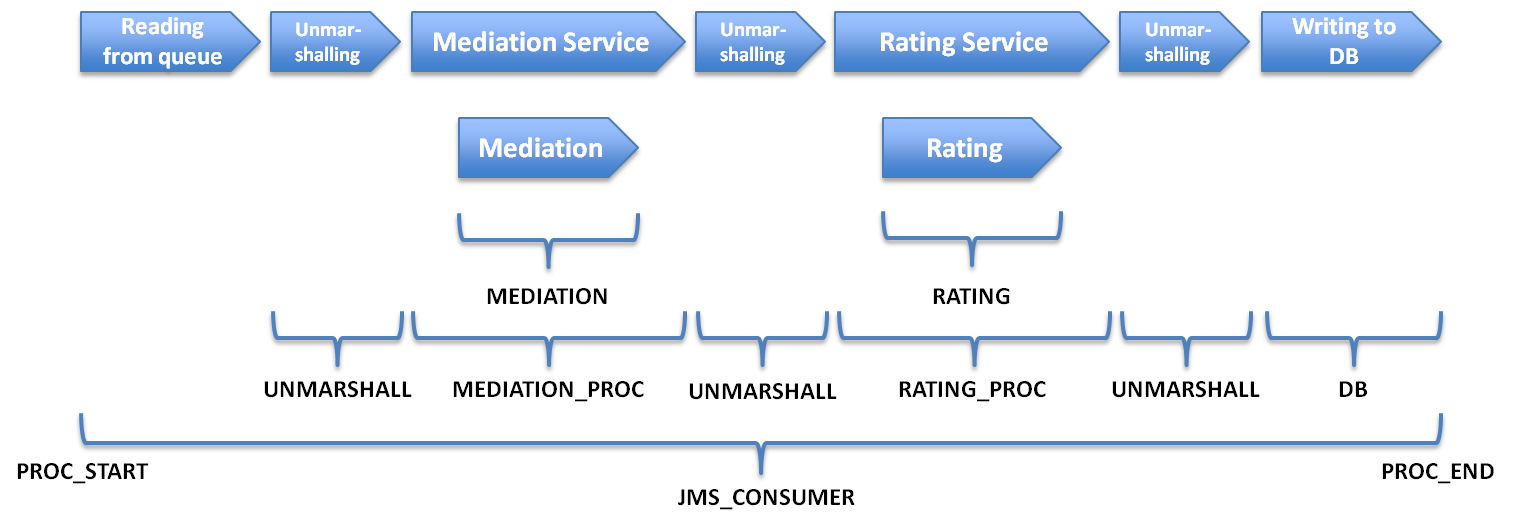
\includegraphics[width=\columnwidth]{measuring_points_messaging}
	\caption{Measuring points of the messaging prototype}
	\label{fig:ch4_measuring_points_messaging}
\end{figure}

A detailed description of each point is shown in Table \ref{table:ch4_measuring_points_batch} and \ref{table:ch4_measuring_points_messaging}.

\begin{table}
	%\renewcommand{\arraystretch}{1.3}
	\caption{Measuring points of the batch prototype}
	\label{table:ch4_measuring_points_batch}
	\centering
	\begin{tabular}{|l|p{5cm}|}
		\hline
		\bfseries Measuring point & \bfseries Description\\
		\hline
		PROC\_START & Timestamp denoting the start of processing an event\\
		\hline
		PROC\_END & Timestamp denoting the end of processing an event\\
		\hline
		FILE\_READ & Elapsed time for reading events from file\\
		\hline
		MEDIATION & Elapsed time used by the mediation component\\
		\hline
		FILE\_WRITE & Elapsed time for writing events to file\\
		\hline
		FTP & Elapsed time for file transfer using FTP\\
		\hline
		RATING & Elapsed time used by the rating component\\
		\hline
		DB & Elapsed time for writing event to the database\\
		\hline 
	\end{tabular}
\end{table}

\begin{table}[htpb]
	\renewcommand{\arraystretch}{1.5}
	\caption{Measuring points of the messaging prototype}
	\label{table:ch4_measuring_points_messaging}
	\centering
	\begin{tabular}{|l|p{4.5cm}|}
		\hline
		\bfseries Measuring point & \bfseries Description\\
		\hline
		PROC\_START & Timestamp denoting the start of processing an event\\
		\hline
		PROC\_END & Timestamp denoting the end of processing an event\\
		\hline
		JMS\_CONSUMER & Elapsed time processing a single event\\
		\hline
		UNMARSHALL & Elapsed time for unmarshalling an event\\
		\hline
		MEDIATION\_PROC & Elapsed time needed for calling the mediation service\\
		\hline
		MEDIATION & Elapsed time used by the mediation component\\
		\hline
		RATING\_PROC & Elapsed time needed for calling the rating service\\
		\hline
		RATING & Elapsed time used by the rating component\\
		\hline
		DB & Elapsed time for writing event to the database\\
		\hline 
	\end{tabular}
\end{table}

\subsection{Instrumentation}
A logging statement for each measuring point has been added at the appropriate code location of the prototypes using different techniques.

\begin{enumerate}
	\item \textbf{Directly in the code}\\Whenever possible, the logging statements have been inserted directly in the code. This has been the case, when the code that should be measured, has been written exclusively for the protoype, for example the mediation and rating components.
	\item \textbf{Delegation}\\When the code to instrument has been part of a framework that is configurable using Spring, an instrumented delegate has been used.
	\item \textbf{AOP}\\Finally, when the code that should get instrumented was part of a framework that was not configurable using Spring, the logging statements have been added using aspects, which are woven into the resulting class files using AspectJ.
\end{enumerate}

\subsection{Test environment}
\label{sec:ch4_test_environment}

The two prototypes have been deployed to an Amazon EC2 environment to conduct the performance evaluation, with the characterics described in Table \ref{table:ch4_amazon_ec2}.

\subsubsection{Batch prototype}

The batch prototype comprises two EC2 nodes, the \emph{Mediation Node} and the \emph{Rating Node}, containing the \emph{Mediation Batch} and the \emph{Rating Batch}, respectively. The \emph{Costed Event Database} is hosted on the \emph{Rating Node} as well. Figure \ref{fig:ch4_batch_deployment_model} shows the deployment diagramm of the Batch prototype.

\begin{figure}[htbp]
	\centering
	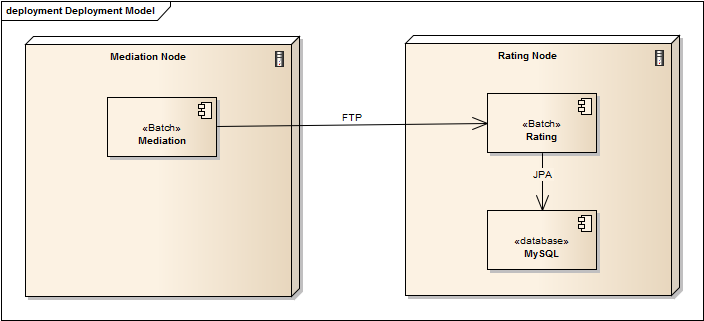
\includegraphics[width=\columnwidth]{batch_deployment_model}
	\caption{Batch prototype deployment on EC2 instances}
	\label{fig:ch4_batch_deployment_model}
\end{figure}

\subsubsection{Messaging Prototype}

The messaging prototype consists of three EC2 nodes, as shown in Figure \ref{fig:ch4_messaging_deployment_model}. The \emph{Master Node} hosts the \emph{ActiveMQ Server} which runs the JMS queue containining the billing events, the \emph{Billing Route}, which implements the processing flow of the prototype and the \emph{MySQL Database} containing the \emph{Costed Event Database}. The \emph{Mediation Node} and \emph{Rating Node} are containing the \emph{Mediation Service} and \emph{Rating Service}, respectively, with each service running inside an Apache Tomcat container.

\subsection{Clock Synchronization}

The clocks of the \emph{Mediation Node} and \emph{Rating Node} are synchronized with the clock of the \emph{Master Node} using PTPd \citep{ptpd}, an implementation of the \ac{PTP} \citep{IEEE_PTP}. The clock of the \emph{Master Node} itself is synchronised with a public timeserver using the \ac{NTP}. Using this approach, a sub-millisecond precision is achieved.

\begin{figure}[htbp]
	\centering
	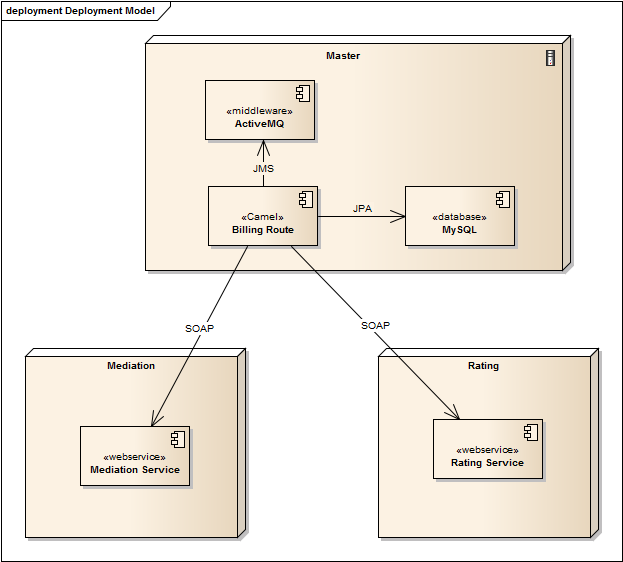
\includegraphics[width=\columnwidth]{messaging_deployment_model}
	\caption{Messaging prototype deployment on EC2 instances}
	\label{fig:ch4_messaging_deployment_model}
\end{figure}

\begin{table}[htbp]
	\renewcommand{\arraystretch}{1.3}
	\caption{Amazon EC2 instance configuration}
	\label{table:ch4_amazon_ec2}
	\centering
	\begin{tabular}{|l|p{3.5cm}|}
		\hline
		\bfseries Instance type & M1 Extra Large (EBS optimized)\\
		\hline
		\bfseries Memory & 15 GiB\\
		\hline
		\bfseries Virtual Cores & 8 (4 cores x 2 units)\\
		\hline
		\bfseries Architecture & 64-bit\\
		\hline
		\bfseries EBS Volume & 10 GiB (100 IOPS)\\
		\hline
		\bfseries Instance Store Volumes & 1690 GB (4x420 GB Raid 0)\\
		\hline
		\bfseries Operating System & Ubuntu 12.04 LTS\\
		& (GNU/Linux 3.2.0-25-virtual x86\_64)\\
		\hline 
		\bfseries Database & MySQL 5.5.24\\
		\hline
		\bfseries Messaging Middleware & Apache ActiveMQ 5.6.0\\
		\hline
	\end{tabular}
\end{table}

\subsection{Preparation and execution of the performance tests}
For running the performance tests, the Master Data DB has been set up with a list of customers, accounts, products and tariffs with each prototype using the same database and data. While part of the testdata like the products and tariffs have been created manually, the relationship between the customers and the products have been generated by a test data generator.

After setting up the master data, a number of test runs have been executed using different sizes of test data (1.000, 5.000, 10.000, 50.000, 100.000, 500.000, 1.000.000 records). To get reliable results, each test configuration has been run three times. Out of the three runs for each configuration, the run having the median processing time has been used for the evaluation.

For each test run, the following steps have been executed:
\begin{enumerate}
	\item \textbf{Generating test data}\\In case of the batch prototype, the event generator writes the test data to file. In case of the messaging prototype, the event generator writes the test data to a \ac{JMS} queue.
	\item \textbf{Running the test}\\Each prototype listens on the file system and the \ac{JMS} queue, respectively. Using the batch prototype, the processing starts when the input file is copied to the input folder of the mediation batch application by the event genarotor. Using the messaging prototype, the processing starts when the first event is written to the JMS queue by the test generator.
	\item \textbf{Validating the results}\\Processsing the log files written during the test run
	\item \textbf{Cleaning up}\\Deleting the created costed events from the DB.
\end{enumerate}

Before running the tests, each prototype has been warmed up by processing 10.000 records.

\subsection{Results} \label{sec:ch4_results}
The performance evaluation yields the following results.

\subsubsection{Throughput}

The throughput per second for a test run with $N$ records is defined as
\begin{displaymath}
{TP/s}_N = N / PT_N
\end{displaymath}
with $PT_N$ being the total processing time for $N$ records. 
Figure \ref{fig:ch4_result_throughput} shows the measured throughput of the batch and messaging prototypes. The messaging prototype is able to process about 70 events per second. The maximum throughput of the batch prototype is about 383 records per second which is reached with an input of 1.000.000 records.

\begin{figure}[htbp]
	\centering
	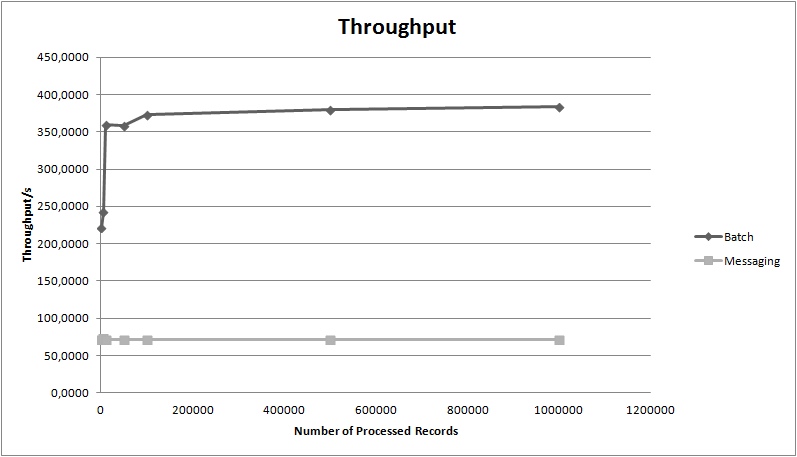
\includegraphics[width=\columnwidth]{throughput_result}
	\caption{Throughput}
	\label{fig:ch4_result_throughput}
\end{figure}

\subsubsection{Latency}\label{sec:result_latency}

Figure \ref{fig:ch4_result_latency} shows the measured latencies of the batch and messaging prototypes. To rule out peaks, the 95th percentile has been used, that is, 95\% of the measured latencies are below this value. In case of the batch prototype, the 95th percentile latency is a linear function of the amount of data. The latency increases proportionally to the number of processd records. In case of the messaging prototype, the 95th percentile latency is approximately a constant value which is independant of the number of processed records.

\begin{figure}[htbp]
	\centering
	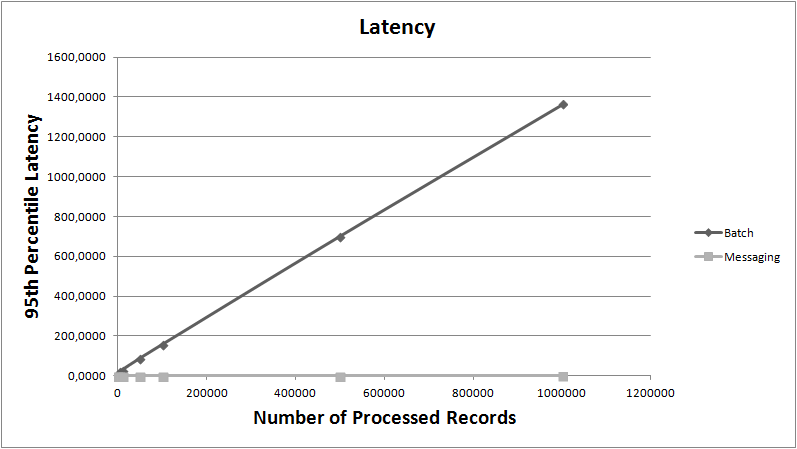
\includegraphics[width=\columnwidth]{latency_result}
	\caption{Latency}
	\label{fig:ch4_result_latency}
\end{figure}

\subsubsection{Processing overhead}

The overhead of the batch prototype is about 7\% of the total processing time, independant of the number of processed records, as shown in Figure \ref{fig:ch4_overhead_batch}. This overhead contains file operations, such as opening, reading, writing and closing of input files, the file transfer between the Mediation and Rating Nodes and the database transactions to write the the processed event to the Costed Events DB.

\begin{figure}[htbp]
	\centering
	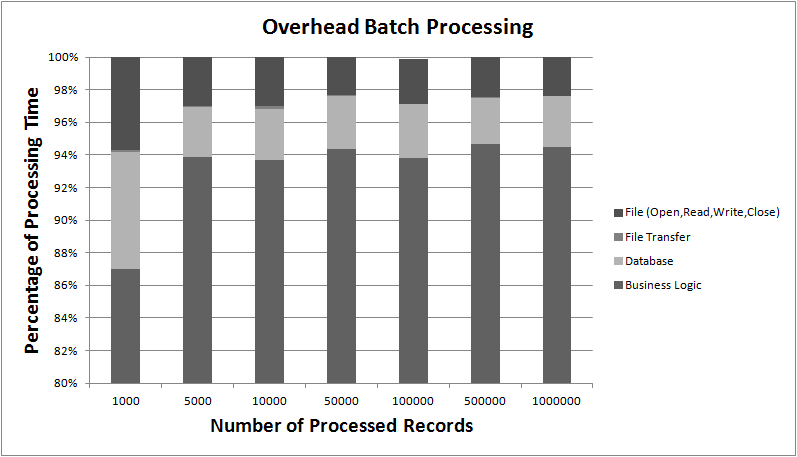
\includegraphics[width=\columnwidth]{overhead_batch}
	\caption{Overhead batch prototype}
	\label{fig:ch4_overhead_batch}
\end{figure}

On the contrary, the overhead of the messaging prototype is about 84\% of the total processing time (see Figure \ref{fig:ch4_overhead_messaging}). In case of the messaging prototype, the overhead contains the JMS overhead, that is the overhead for reading events from the message queue, the webservice overhead needed for calling the Mediation and Rating services including marshalling and unmarshalling of input data and the overhead caused the database transactions to write the processed events to the Costed Events DB. Most of the overhead is induced by the webservice overhead and the database overhead. Since every event is written to the database in its own transaction, the database overhead of the messaging prototype is much larger than the database overhead of the batch prototype.

\begin{figure}[htbp]
	\centering
	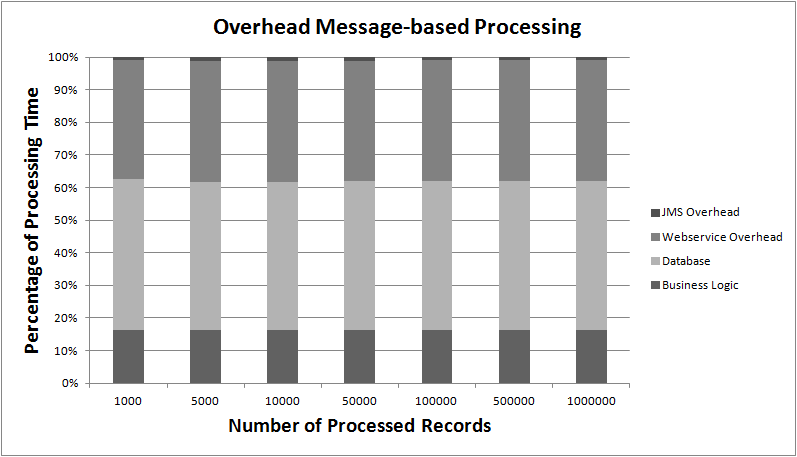
\includegraphics[width=\columnwidth]{overhead_messaging}
	\caption{Overhead messaging prototype}
	\label{fig:ch4_overhead_messaging}
\end{figure}

\subsubsection{System utilisation}

\begin{figure}[htbp]
	\centering
	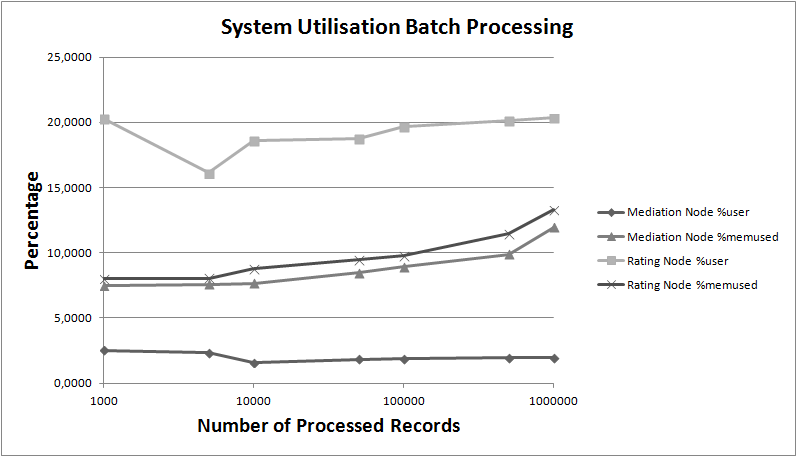
\includegraphics[width=\columnwidth]{systemutilisation_batch}
	\caption{System utilisation batch prototype}
	\label{fig:ch4_systemutilisation_batch}
\end{figure}

The system utilisation has been measured using the sar (System Activity Report) command while running the performance tests. Figure \ref{fig:ch4_systemutilisation_batch} shows the mean percentage of CPU consumption at the user level (\%user) and the mean percentage of used memory (\%memused) for the Mediation node and Rating node of the Batch prototype.
The CPU utilisation of Medation Node and Ratig Node is about 2\% and 19\%, respectively. The memory utilisation increases slowly with the number of processed records.

Figure \ref{fig:ch4_systemutilisation_messaging} shows the mean CPU consumption and mean memory usage for the nodes of the Messaging prototype. The CPU utilisation of the Master Node, Mediation Node and Rating Node is about 9\%, 1\% and 6\%, respectively.
As the same with the batch prototye, the memory utilisation of the messaging prototype increases with the number of processed records. The memory utilisation of the master node peaks at about 38\% with 500000 processed records.
With 1000000 processed records, the memory utilisation is only about 25\%, which presumably can be accounted to the garbage collector.

\begin{figure}[htbp]
	\centering
	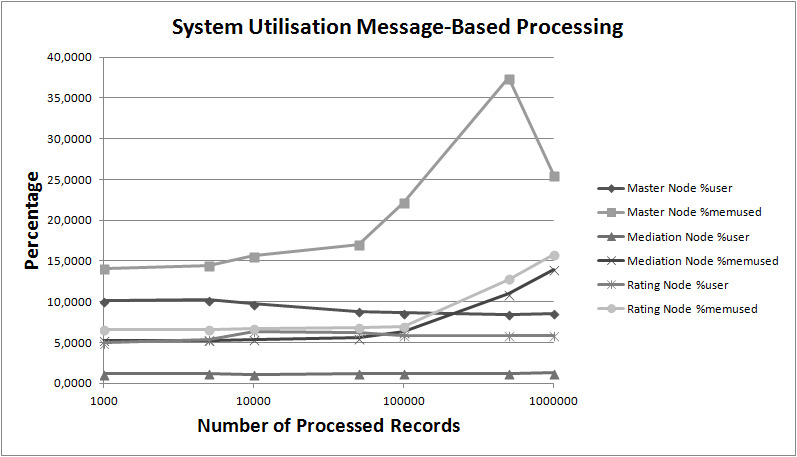
\includegraphics[width=\columnwidth]{systemutilisation_messaging}
	\caption{System utilisation messaging prototype}
	\label{fig:ch4_systemutilisation_messaging}
\end{figure}

\section{Impact of data granularity on throughput and latency}\label{sec:ch4_impact_granularity}
The results presented in Section \ref{sec:ch4_results} suggest that the throughput of the messaging prototype can be increased by increasing the granularity of the data that is beeing processed. Data granularity relates to the amount of data that is processed in a unit of work, for example in a single batch run or an event.
In order to examine this approach, we have repeated the performance tests using different package sizes for processing the data.

\begin{figure}[htbp]
	\centering
	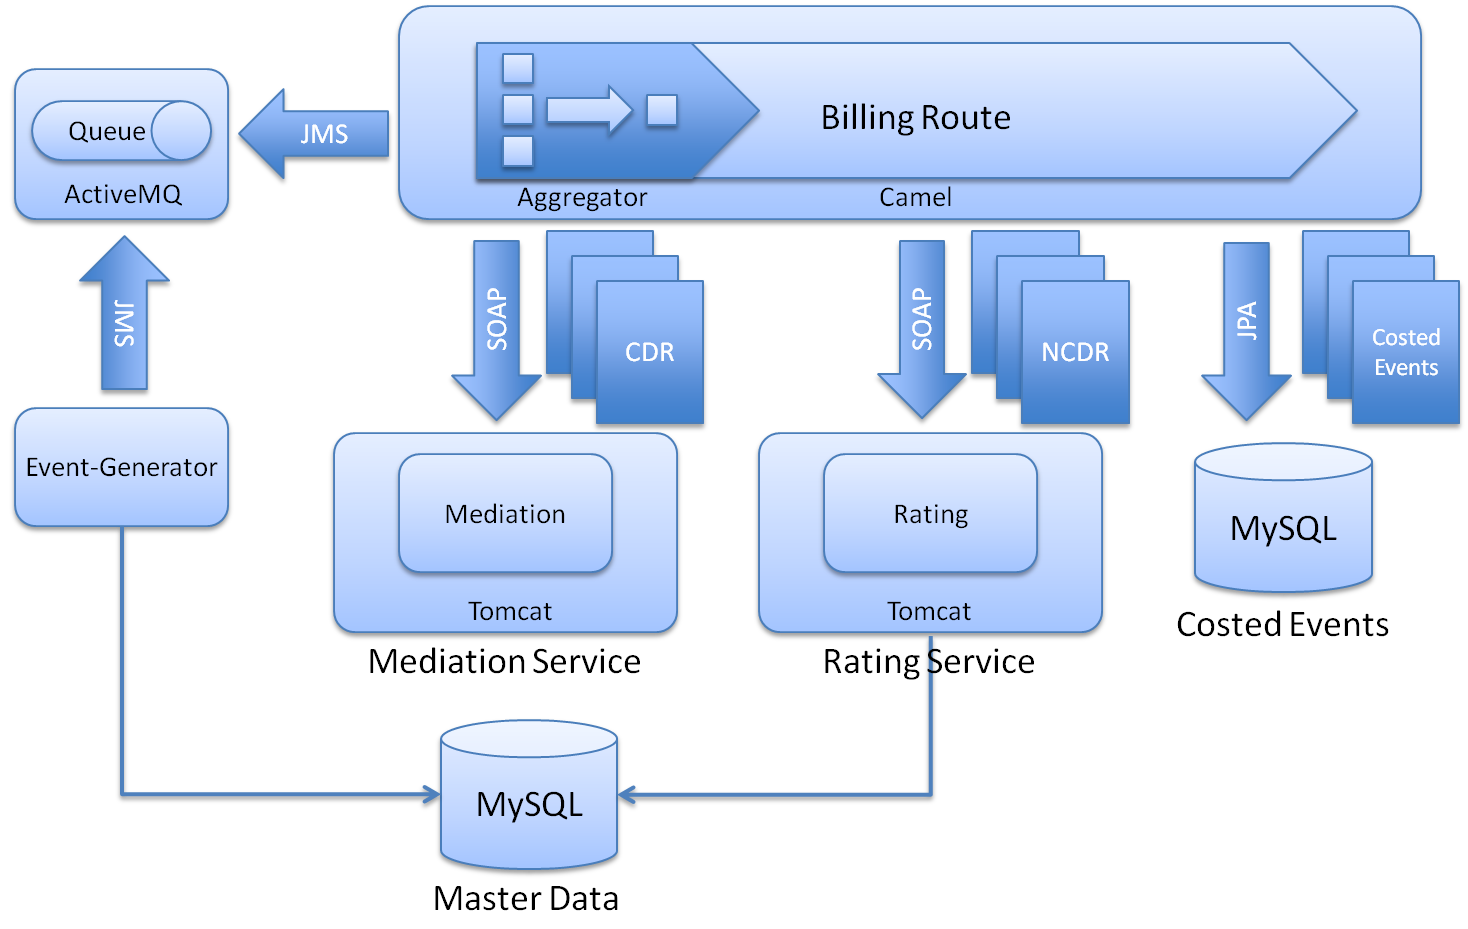
\includegraphics[width=\columnwidth]{messaging_prototype_aggregator}
	\caption{The data granularity is controlled by an aggregator}
	\label{fig:ch4_messaging_prototype_aggregator}
\end{figure}

For this purpose, the messaging prototype has been extended to use an aggregator in the messaging route. The aggregator is a stateful filter which stores correlated messages until a set of messages is complete and sends this set to the next processing stage in the messaging route. In case of the messaging prototype, messages are not corelated to each other and also the messages can be processed in an arbitrary order. A set of messages is complete when it reaches the configured package size. In other scenarios, it is possible to corelate messages by specific data, for example an account number or by a business rule.

Listing \ref{listing:ch4_billing_route_aggregator} shows the definition of the billing route using the aggregator processor, which is provided by Apache Camel (line 7). The aggregator is configured using the correlation expression \lstinline$constant(true)$, which simply aggregates messages in order of their arrival and the aggregation strategy \lstinline$UsageEventsAggrationStrategy$, which implements the merging of incoming messages with already merged messages. The aggregation size is set by \lstinline$completionSize$. The specific value is set in a configuration file. As a fallback, \lstinline$completionTimeout$ defines a timeout in milliseconds to send the set of aggregated messages to the next processing stage before it has reached the defined aggregation size. \lstinline$parallelProcessing$ indicates that the aggregator should use multiple threads (default is 10) to process the finished sets of aggregated messages.

\begin{lstlisting}[caption={Billing route definition with an additional aggregator},label=listing:ch4_billing_route_aggregator]
public void configure() {
		
	errorHandler(deadLetterChannel("activemq:queue:BILLING.ERRORS"));
	
	from("activemq:queue:BILLING.USAGE_EVENTS")
		.unmarshal("jaxbContext")
		.aggregate(constant(true), new UsageEventsAggrationStrategy()).completionSize(completionSize).completionTimeout(completionTimeout).parallelProcessing()
		.to("cxf:bean:mediationEndpoint?dataFormat=POJO&headerFilterStrategy=#dropAllMessageHeadersStrategy&defaultOperationName=processEvents")
		.process(new ProcessEventsPostProcessor())
		.to("cxf:bean:ratingEndpoint?dataFormat=POJO&headerFilterStrategy=#dropAllMessageHeadersStrategy&defaultOperationName=processCallDetails")
		.process(new ProcessCallDetailsPostProcessor())
		.process(costedEventsProcessor);
}
\end{lstlisting}

Figure \ref{fig:ch4_throughput_aggregation} shows the impact of different aggregatation sizes on the throughput of the messaging prototype. For each test 100.000 events have been processed.
\begin{figure}[htbp]
	\centering
	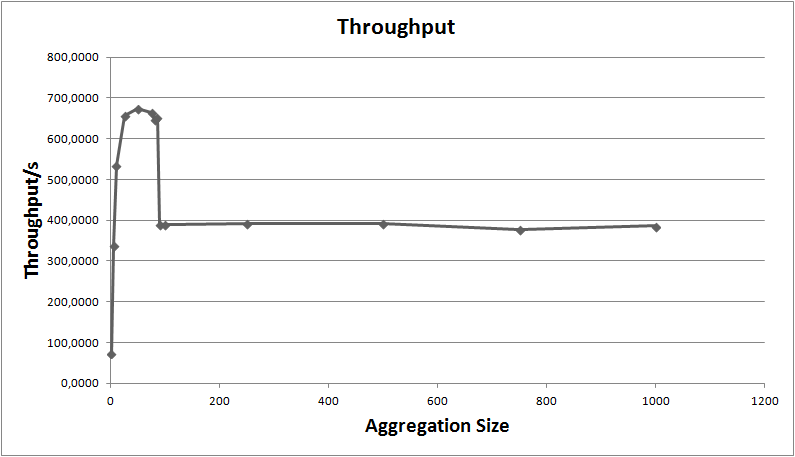
\includegraphics[width=\columnwidth]{throughput_aggregation}
	\caption{Impact of different aggregation sizes on throughput}
	\label{fig:ch4_throughput_aggregation}
\end{figure}
The throughput increases constantly for $1<aggregation\_size<=50$ with a maximum of 673 events per second with $aggregation\_size=50$. Higher aggregation sizes than 50 do not further increase the throughput, it stays around 390 events per second. Surprisingly, the maximum throughput of 673 events per second even outperforms the throughput of the batch prototype which is about 383 records per second. This is presumably a result of the better multithreading capabilities of the camel framework.

Increasing the aggregation size also decreases the processing overhead, as shown in Figure \ref{fig:ch4_overhead_aggregation}. An aggregate size of 10 decreases the overhead by more than 50\% compared to an aggregate size of 1. Of course, the integration of the aggregator adds an additional overhead which is insignificant for $aggregation\_size>50$.
\begin{figure}[htbp]
	\centering
	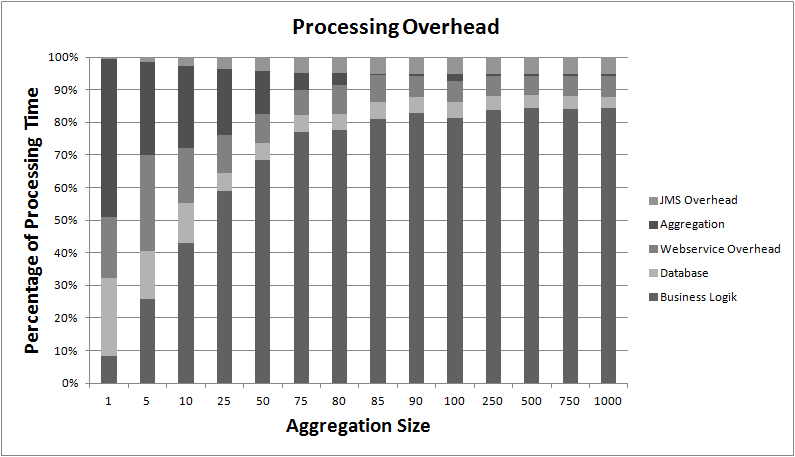
\includegraphics[width=\columnwidth]{overhead_aggregation}
	\caption{Impact of different aggregation sizes on processing overhead}
	\label{fig:ch4_overhead_aggregation}
\end{figure}

The increased throughput achieved by increasing the aggregation size comes with the cost of a higher latency. Figure \ref{fig:ch4_latency_aggregation} shows the impact of different aggregation sizes on the 95th percentile latency of the messaging prototype. 
\begin{figure}[htbp]
	\centering
	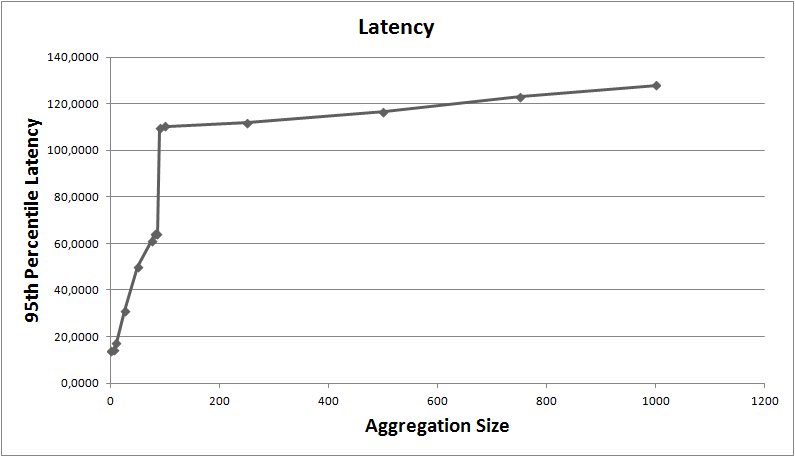
\includegraphics[width=\columnwidth]{latency_aggregation}
	\caption{Impact of different aggregation sizes on latency}
	\label{fig:ch4_latency_aggregation}
\end{figure}

An aggregation size of 50, resulting in the maximum throughput of 673 events per seconds, shows a 95th percentile latency of about 68 seconds. This latency is significantly higher than the latency of the messaging system without message aggregation, which is about 0,15 seconds (see Section \ref{sec:result_latency}).

The results indicate that there is an optimal range for the aggregation size to control the throughput and latency of the system. Setting the aggregation size higher than a certain threshold leads to a throughput drop and latency gain. In case of our prototype, this threshold is between an aggregation size of 85 and 90. The observed throughput drop and latency gain is caused by a congestion in the aggregator. Messages are read faster from the queue than they are getting processed by the aggregator.

Figure \ref{fig:ch4_systemutilisation_aggregation} shows the impact of different aggregation sizes on the system utilisation. The CPU utilisation of the Master node shows a maximum of 30\% with an aggregation size of 25. An $aggregation\_size >= 90$ results in a CPU utilisation of about 15\%. The maximum memory utilisation of the Master node is 41\% with an aggregation size of 100.

The maximum system utilisation of the Rating node is 25\% with an aggregation size of 80. The memory utilisation is between 7-8\% irrespective of aggregation size. Maximum system and memory utilisation of the Mediation node are also irrespective of aggregation size, beeing less than 2\% and 8\%, respectively.

\begin{figure}[htbp]
	\centering
	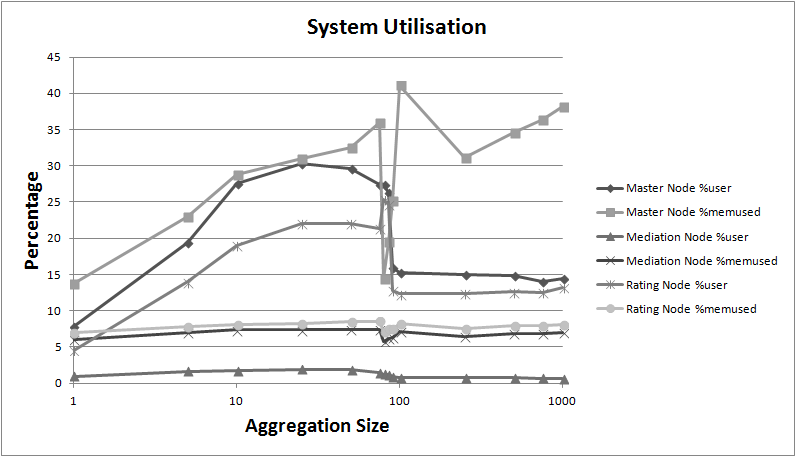
\includegraphics[width=\columnwidth]{systemutilisation_aggregation}
	\caption{Impact of different aggregation sizes on system utilisation}
	\label{fig:ch4_systemutilisation_aggregation}
\end{figure}

When using high levels of data granularity, the messaging system is essentially a batch processing system, providing high throughput with high latency. To provide near-time processing an optimum level of data granularity would allow having the lowest possible latency with the lowest acceptable throughput.

\section{Discussion with respect to related work}\label{sec:ch4_related_work}
\todo[inline]{Discuss why a prototype has been built instead of using a model of the system.}
This section gives an overview of work related to the research presented in this paper. Related work can be categorised in two different topics, performance measuring and performance optimisation of messaging systems. Performance measuring is applied to evaluate if an implemented system meets its performance requirements and to spot possible performance problems. Performance optimisation aims to improve the performance of a system to meet certain requirements such as throughput or latency.

\subsection{Performance Measuring}
Her et al. \citep{Her:2007qf} propose the following set of metrics for measuring the performance of a service-oriented system:
\begin{itemize}
	\item \textbf{Service response time}\\
	Elapsed time between the end of request to service and the beginning of the response of the service. This metric is further split in 20 sub-metrics such as message processing time, service composition time and service discovery time.
	\item \textbf{Think time}\\
	Elapsed time between the end of a response generated by a service and the beginning of a response of an end user.
	\item \textbf{Service tournaround time}\\
	Time needed to get the result from a group of related activities within a transaction.
	\item \textbf{Throughput}\\
	Number of requests served at a given period of time. The authors distinguish between the throughput of a service and the throughput of a business process.
\end{itemize}

In their work, \cite{Henjes:2006nx}\cite{Menth:2006ys} investigated the throughput performance of the JMS server FioranaMQ, SunMQ and WebsphereMQ. The authors came to the following conclusion:
\begin{itemize}
	\item Message persistence reduces the throughput significantly.
	\item Message replication increases the overall throughput of the server.
	\item Throughput is limited either by the processing logic for small messages or by the transmission capacity for large messages.
	\item Filtering reduces the throughput significantly.
\end{itemize}

\cite{Chen:2004cr} propose that the following performance metrics should be used to evaluate a JMS server:
\begin{itemize}
	\item Maximum sustainable throughput
	\item Latency
	\item Elapsed time taken to send batches messages
	\item Persistent message loss after recovery
\end{itemize}
The authors state that ``although messaging latency is easy to understand, it is difficult to measure precisely in a distributed environment without synchronised high- precision clocks.'' They discovered that latencies increase with increasing message sizes.

SPECjms2007 is a standard benchmark for the evaluation of Message-Oriented Middleware platforms using \ac{JMS} \citep{Sachs:2009rr}. It provides a flexible performance analysis framework for tailoring the workload to specific user requirements. According to \cite{sachs2007designing}, the workload of the SPECjms2007 benchmark has to meet the following requirements:
\begin{itemize}
	\item \textbf{Representativeness}\\
	The workload should reflect how the messaging platform is used in typical user scenarios.
	\item \textbf{Comprehensiveness}\\
	The workload should incorporate all platform features typically used in JMS application including publish/subscript and point-to-point messaging.
	\item \textbf{Focus}\\
	The workload should focus on measuring the performance of the messaging middleware and should minimize the impact of other components and services.
	\item \textbf{Configurability}\\
	It should be possible to configure the workload to meet the requirements of the user.
	\item \textbf{Scalability}\\
	It should be possible to scale the workload by the number of destinations with a fixed traffic per destination or by increasing the traffic with a fixed set of destinations.
\end{itemize}

\cite{Ueno:2006ly} propose a methodology to evaluate the performance of an ESB in an early stage of development that can be used for capacity planning. Instead of using a performance model for performance prediction, they run the ESB on a real machine with a pseudo-environment using lightweight web service providers and clients. The authors state that model-based approaches ``often require elemental performance measurements and sophisticated modeling of the entire system, which is usuable not feasible for complex systems''.

\subsection{Performance Optimisation}
\todo[inline]{Most of this section should be moved to Section \ref{ch:03_related_work}}
Various approaches have been proposed to optimise the performance of webservices, in particular SOAP, the standard protocol for Web Service communication. This includes approaches for optimising the processing of SOAP messages (see for example \cite{Abu-Ghazaleh:2005bs}, \cite{Suzumura:2005fv} and \cite{Ng:2006kl}), compression of SOAP messages (see for example \cite{Estrella:2008dz} and \cite{Ng:2005qa}) and caching (see for example \cite{andresen2004lye} and \cite{Devaram:2003fu}). A survey of the current approaches to improve the performance of SOAP can be found in \cite{Tekli:2012bh}.

\cite{Wichaiwong:2007oq} propose an approach to transfer bulk data between web services per FTP. The SOAP messages transferred between the web services would only contain the necessary details how to download the corresponding data from an FTP server since this protocol is optimized for transferring huge files. This approach solves the technical aspect of efficiently transferring the input and output data but does not pose any solutions how to implement loose coupling and how to integrate heterogeneous technologies, the fundamental means of an SOA to improve the flexibility of an application landscape.

Data-Grey-Box Web Services are an approach to transfer bulk data between Web Services \citep{Habich:2007ij}. Instead of transferring the data wrapped in SOAP messages, it is transferred using an external data layer. For example when using database systems as data layer, this facilitates the use of special data transfer methods such \ac{ETL} to transport the data between the database of the service requestor and the database of the Web service. The data transfer is transparent for both service participants in this case. The approach includes an extension of the Web service interface with properties describing the data aspects. Compared to the SOAP approach, the authors measured a speedup of up to 16 using their proposed approach. To allow the composition and execution of Data-Grey-Box Web services, \cite{Habich:kl} developed BPEL data transitions to explicitly specify data flows in BPEL processes.

\cite{Zhuang:2012qf} propose three tuning strategies to improve the performance of \ac{JMS} for cloud-based applications.
\begin{enumerate}
	\item When using persistent mode for reliable messaging the storage block size should be matched with the message size to maximise message throughput.
	\item Applying distributed persistent stores by configuring multiple JMS destinations to achieve parallel processing
	\item Choosing appropriate storage profiles such as RAID-1
\end{enumerate}

MPAB (Massively Parallel Application Bus) is an ESB-oriented messaging bus used for the integration of business applications \citep{Benosman:2012zr}. The main principle of MPAB is to fragment an application into parallel software processing units, called SPU. Every SPU is connected to an Application Bus Multiplexor (ABM) through an interface called Application Bus Terminal (ABT). The Application Bus Multiplexor manages the resources shared across the host system and communicates with other ABM using TCP/IP. The Application Bus Terminal contains all the resources needed by SPU to communicate with its ABM. A performance evaluation of MPAB shows that it achieves a lower response time compared to the open source ESBs Fuse, Mule and Petals.

Some research has been done to add real-time capabalities to ESB or messaging middleware. \cite{Garces-Erice:2009kx} proposes an architecture for a real-time messaging middleware based on an Enterprise Service Bus. It consists of an event scheduler, a \ac{JMS}-like API and a communication subsystem. While fulfilling real-time requirements, the middleware also supports already deployed infrastructure.

In their paper, \cite{Xia:2011rt} suggest a real-time ESB model by extending the JBI specification with semantics for priority and time restrictions and modules for flow control and bandwith allocation. The proposed system is able to dynamically allocate bandwidth according to business requirements.

Tempo is a real-time messaging system written in Java that can be used on either a real-time or non-real-time architecture \citep{Bauer:2008fk}. The authors, Bauer et al., state that existing messaging systems are designed for transactional processing and therefore not appropriate for applications with with stringent requirements of low latency with high throughtput. The main principle of Tempo is to use an independent queuing system for each topic. Ressources are partitioned between these queueing systems by a messaging scheduler using a time-base credit scheduling mechanism. In a test environment, Tempo is able to process more than 100.000 messages per second with a maximum latency of less than 120 milliseconds.

\cite{Haesen:2008ve} distinguishes between two types of data granularity:
\begin{itemize}
	\item \textbf{Input data granularity}\\
	Data that is sent to a component
	\item \textbf{Output data granularity}\\
	Data that is returned by a component
\end{itemize}
The authors state that a coarse-grained data granularity reduces the communication overhead, since the number of network transfers is decreased.
``Especially in the case of Web services, this overhead is high since asynchronous messaging requires multiple queuing operations and numerous XML transformations''.

\todo[inline]{Discuss contributions in this chapter with respect to related work. What is different?}


\section{Summary}\label{sec:ch4_summary}
Near-time processing of bulk data is hard to achieve. As shown in Section \ref{sec:ch2_latency_throughput}, latency and throughput are opposed performance metrics of a system for bulk data processing. Batch processing, while providding high throughput, leads to high latency, which impedes near-time processing. Message-base processing delivers low latency but cannot provide the throughput for bulk data processing due to the additional overhead for each processed message.

While it is technically possible to minimise the overhead of a messaging system by implementing a lightweight marshalling system and not use JMS or other state-of-the-art technologies such as XML, SOAP or REST, it would hurt the ability of the messaging middleware to integrate heterogenous systems or services and thus limiting its flexibility, which is one the main selling propositions of such a middleware. Furthermore, batch processing enables optimizations by partitioning and sorting the data appropriately which is not possible when each record is processed independently as a single message.

In order to compare throughput and latency of batch and message-oriented systems, a prototype for each processing type has been built. A performance evaluation has been conducted with the following results:
\begin{itemize}
	\item The throughput of the batch prototype is 4 times the throughput of the messaging prototype.
	\item The latency of the messaging prototype is only a fraction of the latency of the batch prototype.
	\item The overhead of the messaging prototype is about 84\% of the total processing time, which is mostly induced by the webservice overhead and the database transactions. 
	\item The overhead of the batch prototype is only about 7\% of the total processing time.
\end{itemize}

The results presented in Section \ref{sec:ch4_impact_granularity} show that throughput and latency depend on the granularity of data that is being processed. 
\begin{itemize}
	\item The throughput increases constantly for an aggreation size > 1 and <= 50 with a maximum of 673 events per second with an aggregation size = 50.
	\item The increased throughput achieved by increasing the aggregation size comes with the cost of a higher latency. An aggregation size of 50, resulting in the maximum throughput of 673 events per seconds, shows a 95th percentile latency of about 68 seconds. This latency is significantly higher than the latency of the messaging system without message aggregation, which is about 0,15 seconds.
	\item Increasing the aggregation size also decreases the processing overhead of the messaging prototype. An aggregate size of 10 decreases the overhead by more than 50\% compared to an aggregation size of 1.
	\item There is an optimal range for the aggregation size to control the throughput and latency of the system. Setting the aggregation size higher than a certain threshold leads to a throughput drop and latency gain cause by a congestion in the aggregator.
\end{itemize}

The performance tests that have been run for the evaluation described in section \ref{sec:ch4_evaluation} are static tests, in the sense that they do not take different load scenarios of the system into account. In a real situation, the current throughput and latency also depend on the current load of the system. If the system is not able to handle the current load, messages are congested in the input queue which increases the latency of the system. A higher maximum throughput would decrease the latency in this case. 

Therefore, the aggregation size used by the messaging system should depend on the current load of the system. It is not feasible to find a static aggregation size that works under all load conditions resulting in an optimum latency.

The next chapter presents a solution for this problem. It describes an adaptive middleware that is able to adjust the data aggregation size at runtime, depending on the current load of the system.